\documentclass[12pt]{report}
\usepackage{amsmath}
\usepackage{ragged2e}
\usepackage{graphicx}
\graphicspath{ {./img/} }
\setlength\parindent{0pt}

\begin{document}

\Large
\centering
AMS310 Homework \#1

\justify
\normalsize

Kuba Gasiorowski\\
ID: 109776237\\

\noindent1a) The mean and median of the high temperatures is $\boxed{61.25}$ and $\boxed{61,}$ respectively. The mean and median of the low temperatures is $\boxed{48.25}$ and $\boxed{48.54.}$
\bigskip\\
\noindent b) \\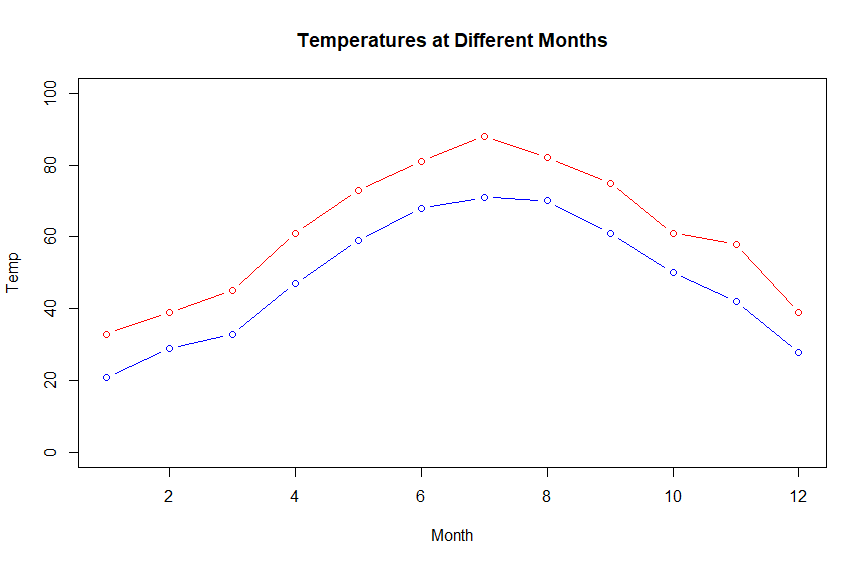
\includegraphics[scale=0.625]{temp} \\

\noindent c) Shortcut formula $ \Rightarrow s^2 = \frac{\sum_{i=1}^n x_i^2 - (\sum_{i=1}^nx_i)^2/n}{n-1}$\\
$\Rightarrow \frac{31395 - (579)^2/12}{12-1}$\\
$\Rightarrow \frac{3458.25}{11}$\\
$\Rightarrow \boxed{314.4}$\

\clearpage

\noindent d) \\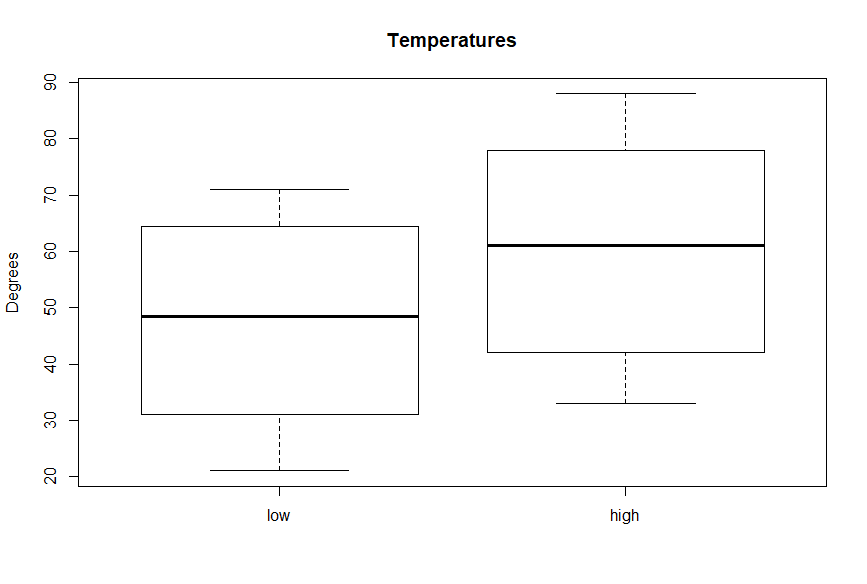
\includegraphics[scale=0.625]{temp_box}\\

\hrulefill
\bigskip

\noindent 2a) Since there are 98 total parasites when accounting for frequencies, the 1st quartile will be entry number 24.5 (rounded up to 25), which is $\boxed{23m.}$ Using the same method, the third quartile will be entry number 73.5 (rounded up to 74) which is $\boxed{26m.}$\\

\noindent b) Sample mean $\Rightarrow \bar{x} = \frac{\sum_{i=1}^n(x_i \cdot f_i)}{\sum_{i=1}^n{f_i}}$\\
$\Rightarrow \frac{2359}{98} \Rightarrow \boxed{24.1}$\\

\noindent c) Same method as part a: median is the 98/2 = 49th entry, which is $\boxed{24m.}$\\

\clearpage

\noindent 3a) 
\begin{verbatim}
> t <- c(29,33,38, ... 94,97,100) # Convert the stem to a vector
> median(t)
[1] 78
\end{verbatim}

\noindent b)
\begin{verbatim}
> quantile(t, .70) # 70th percentile
70% 
85.8
\end{verbatim}
\noindent c)
\begin{verbatim}
> quantile(t, .25) # First quartile
25% 
53.5 
> quantile(t, .75) # Third quartile
75% 
87.5 
> IQR(t) # Interquartile range
[1] 34
\end{verbatim}

\noindent d) An outlier is an observation which is less than $Q_1 - 1.5($IQR$)$ (2.5) or greater than $Q_3 + 1.5($IQR$)$ (138.5). Since there's no score below 2.5, or greater than 138.5, there are no outliers.\\

\clearpage

\noindent 4a) \\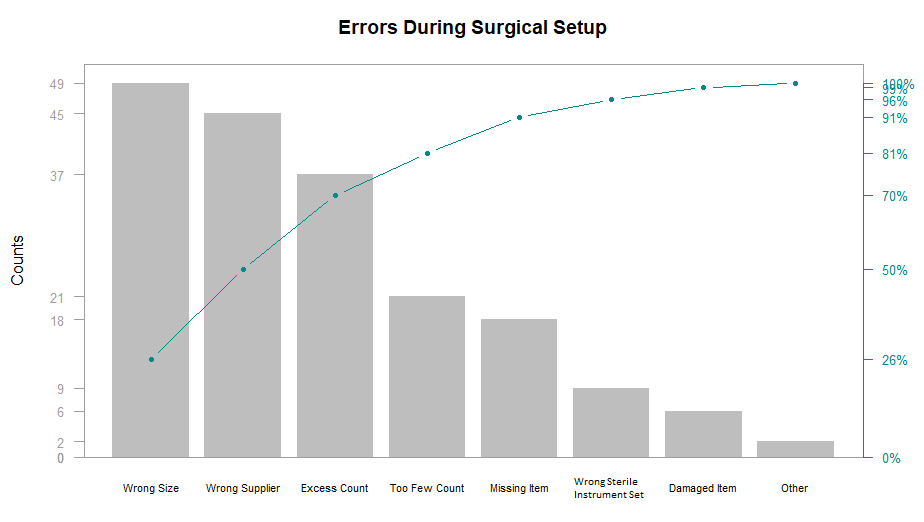
\includegraphics[scale=0.6]{4pareto} 

\scriptsize

(This pareto chart was creating by using the technique found at
 \textbf{https://preview.tinyurl.com/yav7lpu5}) 
\normalsize

\bigskip

\noindent b) From looking at the pareto chart, it is evident that the first four types of error (Wrong size, Wrong Supplier, Excess Count, Too Few Count) account for more than 80\% of all the errors.

\clearpage

\noindent 5a) \\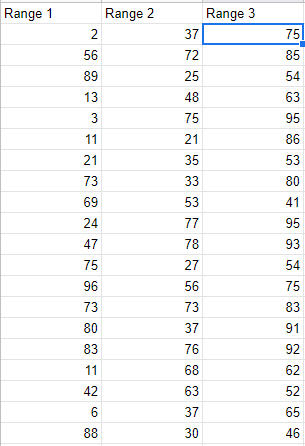
\includegraphics[scale=0.7]{raw_data}

\noindent b) \\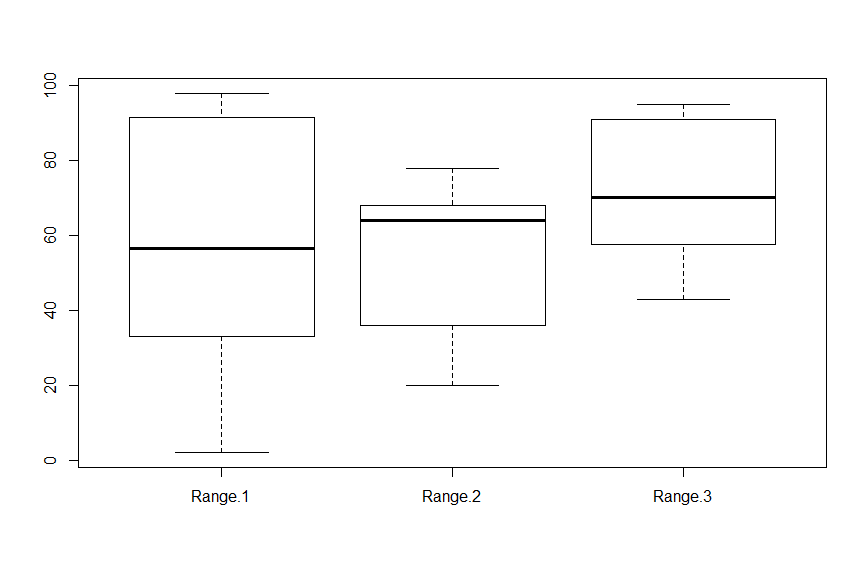
\includegraphics[scale=0.6]{box_plot}

\clearpage

\noindent 6a)

\begin{verbatim}
> d <- c(55, 61, ..., 99, 87)
> hist(d)
\end{verbatim}

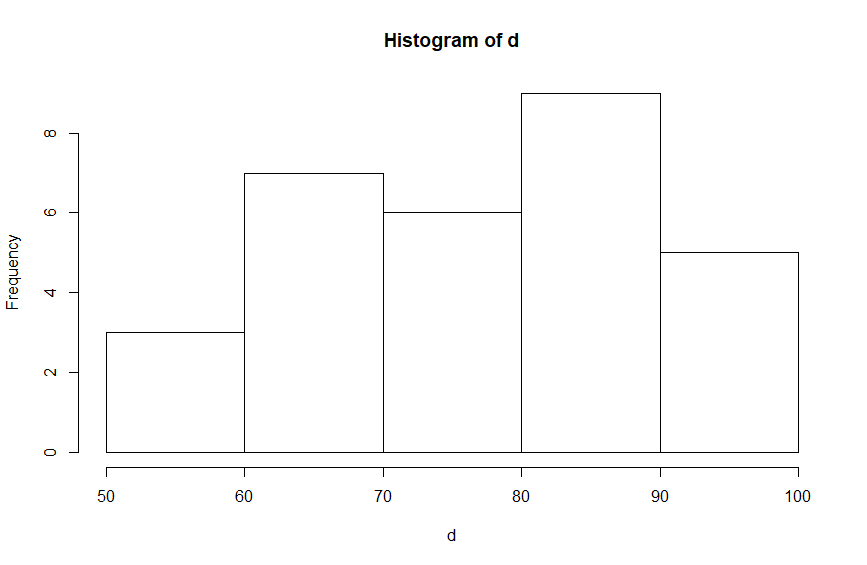
\includegraphics[scale=0.6]{6hist}
\noindent b)
\begin{verbatim}
> mean(d)
[1] 76.63333
> var(d)
[1] 147.8264
\end{verbatim}
\noindent c)
\begin{verbatim}
> summary(d)
Min. 1st Qu.  Median    Mean 3rd Qu.    Max. 
54.00   69.00   77.00   76.63   84.75   99.00
\end{verbatim}

\clearpage

\noindent d)
\begin{verbatim}
> boxplot(d, main="Box plot of data")
\end{verbatim}

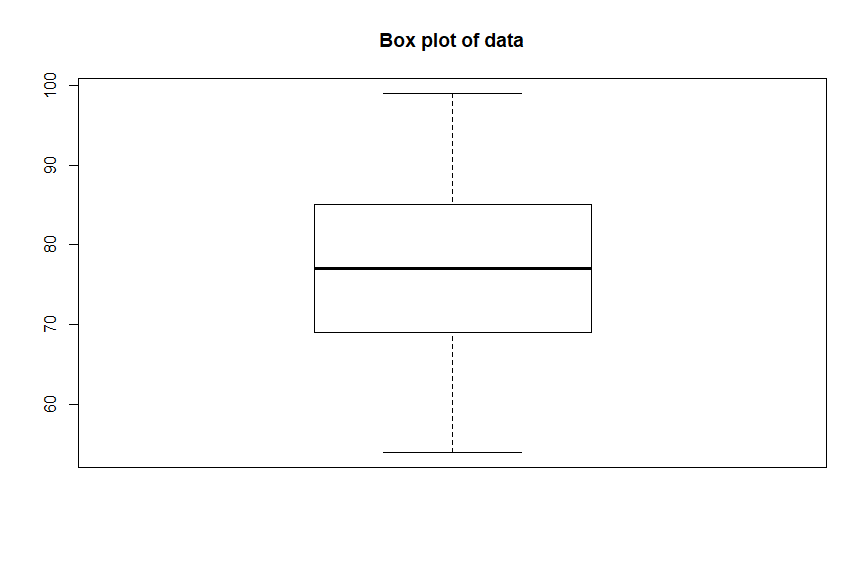
\includegraphics[scale=0.625]{6box}

\noindent e)
\begin{verbatim}
	> stem(d, 0.5)
	
	The decimal point is 1 digit(s) to the right of the |
	
	5 | 459
	6 | 123899
	7 | 0233577
	8 | 111124579
	9 | 22449
\end{verbatim}

\end{document}
